% CSCI 435 Research Track paper -- IEEE conference template.
\documentclass[conference]{IEEEtran}

\usepackage[utf8]{inputenc}
\usepackage[T1]{fontenc}
\usepackage{amsmath,amssymb}
\usepackage{graphicx}
\usepackage{booktabs}
\usepackage{url}
\usepackage[hidelinks]{hyperref}

% Figures are produced by experiments/generate_figures.py into ../figures/.
\graphicspath{{../figures/}{figures/}}

% Measured and computed results quoted in the text come from this generated file;
% parameters, small integers and figures from other papers are typed directly.
% Generated by experiments/generate_figures.py -- do not edit by hand.
\newcommand{\Seed}{435}
\newcommand{\Trials}{20{,}000}
\newcommand{\CoalAkOne}{2/7}
\newcommand{\CoalCkFour}{35/35}
\newcommand{\CoalDkFour}{24/35}
\newcommand{\CoalDkFourFrac}{0.686}
\newcommand{\CoalDkFive}{19/21}
\newcommand{\CoalCthreekThree}{35/35}
\newcommand{\CoalDthreekThree}{12/35}
\newcommand{\CoalCfivekFive}{21/21}
\newcommand{\CoalDfivekFive}{19/21}
\newcommand{\GasApproveEach}{84{,}858}
\newcommand{\GasFinalizeC}{80{,}669}
\newcommand{\GasFinalizeD}{81{,}556}
\newcommand{\GasRoleOverhead}{887}
\newcommand{\GasRoleOverheadPct}{0.18\%}
\newcommand{\GasDeployRegistry}{2{,}508{,}853}
\newcommand{\MissingRoleD}{2.1\%}
\newcommand{\GasTotalA}{198{,}846}
\newcommand{\TxsA}{2}
\newcommand{\CompleteA}{99.0\%}
\newcommand{\OnTimeA}{98.7\%}
\newcommand{\MedianDelayA}{0.71}
\newcommand{\PninetyfiveDelayA}{2.08}
\newcommand{\OutageFiveA}{94.0\%}
\newcommand{\OutageTenA}{89.1\%}
\newcommand{\GasTotalB}{758{,}182}
\newcommand{\TxsB}{8}
\newcommand{\CompleteB}{47.7\%}
\newcommand{\OnTimeB}{42.7\%}
\newcommand{\MedianDelayB}{2.68}
\newcommand{\PninetyfiveDelayB}{6.14}
\newcommand{\OutageFiveB}{40.9\%}
\newcommand{\OutageTenB}{34.8\%}
\newcommand{\GasTotalC}{480{,}981}
\newcommand{\TxsC}{5}
\newcommand{\CompleteC}{99.6\%}
\newcommand{\OnTimeC}{99.5\%}
\newcommand{\MedianDelayC}{1.10}
\newcommand{\PninetyfiveDelayC}{2.22}
\newcommand{\OutageFiveC}{96.8\%}
\newcommand{\OutageTenC}{93.0\%}
\newcommand{\GasTotalD}{481{,}868}
\newcommand{\TxsD}{5}
\newcommand{\CompleteD}{97.6\%}
\newcommand{\OnTimeD}{96.9\%}
\newcommand{\MedianDelayD}{1.22}
\newcommand{\PninetyfiveDelayD}{2.87}
\newcommand{\OutageFiveD}{83.9\%}
\newcommand{\OutageTenD}{71.8\%}


\begin{document}

\title{Design and Evaluation of an Insider-Resistant Blockchain Academic Credential Verification System for Kazakhstan}

\author{
  \IEEEauthorblockN{Daulet Tuleyev and Damir Kushumbayev}
  \IEEEauthorblockA{Department of Computer Science, School of Computing and Artificial Intelligence\\
  Nazarbayev University, Astana, Kazakhstan}
}

\maketitle

\begin{abstract}
A blockchain can show which account registered an academic credential and that the record has not changed since. It cannot show that the account holder was honest. We study issuance as an authorization problem inside one university and ask how role-constrained approval compares with single-issuer, unanimous and role-agnostic threshold approval in insider resistance, gas consumption and availability. We implement a Solidity registry that stores salted commitments and delegates only the issuance decision to an interchangeable policy contract, so that credential format, storage and lifecycle are identical across policies. For a synthetic university with two registrars, three deans and two examination officers we enumerate every insider coalition and check each outcome against the contracts, measure gas from transaction receipts, and simulate approval delay and absence. At a common 4-of-7 threshold, requiring every role leaves the minimum coalition size at four but reduces the capable four-person coalitions from \CoalCkFour{} to \CoalDkFour{}, for \GasRoleOverheadPct{} more gas per issuance. The price is availability: two absent employees can block issuance instead of four, and under a 5\% whole-role outage simulated completion falls from \OutageFiveC{} to \OutageFiveD{}. Larger staffings remove most of the loss from individual absence but not the loss from whole-role outages. The benefit of roles depends on how people collude: under independent compromise with probability 0.1 the role requirement lowers the probability that a compromised set can issue by \CorRedZero{}, and by \CorRedHalf{} when the correlation within offices is 0.5. No policy is best on all measures. We relate the results to diploma verification in Kazakhstan and state what the design cannot prevent, above all a compromised governor and falsified source records.
\end{abstract}

\begin{IEEEkeywords}
blockchain, academic credentials, insider threat, separation of duty, smart contracts, Kazakhstan
\end{IEEEkeywords}

\section{Introduction}\label{sec:intro}
Employers and universities rely on diplomas they did not issue and often cannot check. Blockchain-based systems address part of this problem: the issuer registers a digest of the credential, and any later change to the document no longer matches the record. The guarantee is about integrity after registration. It says nothing about whether the registration itself was legitimate.

That distinction matters when the attacker works for the issuer. Kazakhstan's national anti-corruption report for 2023 describes this situation. It states that about 2,600 university employees had been given rights to edit the national education database used to confirm diplomas, that a further 550 could generate diploma QR codes, and that such powers without effective control created risks of issuing forged diplomas~\cite{kzreport2023}. At 19 inspected universities, 2,733 people were listed in the database but absent from the universities' own records, and the database allowed graduates to be entered retroactively~\cite{kzreport2023}. The report also counts 1,143 diplomas whose issuance the institutions did not confirm~\cite{kzreport2023}; an unconfirmed diploma is not necessarily a forged one. A ledger's timestamps would expose retroactive entry. They would not expose a false entry submitted on time by an authorized account, which the ledger would preserve faithfully.

Recent work on Kazakhstan recognizes the same risk. The system of Ussatova et al.\ treats university administrators as not fully trusted, because they may make errors, misuse privileges or be compromised~\cite{ussatova2026b}. Its answer is to authenticate, authorize and log their operations, and an account with the issuer role can register a record.

The usual response to misuse of authority is separation of duty: no single person can complete a sensitive task~\cite{ferraiolo1992}. Credential systems have adopted parts of this idea through multisignature issuance~\cite{lone2020}, majority voting by nodes~\cite{sarwar2026} and quorums of registrars~\cite{saramago2021}. The idea we evaluate is not new: Cerberus already proposes that a registrar and an examination department should both sign~\cite{tariq2023}, and policies that combine team size with qualifications have been formalized in general~\cite{li2008}. The credential designs differ in threshold, in who may sign and in platform, so their published evaluations do not show what a role requirement adds beyond a larger number of signatures, or what it costs.

\textbf{Gap.} In the work we reviewed, we found no evaluation that holds one credential contract, university and approval threshold fixed and measures how adding a role requirement changes insider-coalition exposure, gas consumption and issuance availability together.

\textbf{Research question.} How do role-constrained approval policies compare with single-issuer, unanimous and threshold policies in insider resistance, gas consumption and credential issuance availability? We divide it into three sub-questions:
\begin{itemize}
\item \textbf{SQ1.} Which coalitions of compromised employees can issue a credential under each policy?
\item \textbf{SQ2.} How much gas does one completed issuance consume?
\item \textbf{SQ3.} How do employee absence and delay affect whether and when a credential is issued?
\end{itemize}

\textbf{Contributions.} The individual mechanisms are known. Our contribution is a controlled comparison of them:
\begin{itemize}
\item a registry with four interchangeable approval policies and an identical credential lifecycle;
\item an exhaustive coalition analysis in which all 1,016 outcomes were also executed against the contracts;
\item a gas comparison from receipts, with the threshold and signers held equal for the two policies of main interest;
\item a simulation of absence and delay, together with the exact number of absences that blocks each policy;
\item an exact study of other staffings and of collusion correlated within offices; and
\item a discussion of deployment beside Kazakhstan's existing verification platform.
\end{itemize}

\section{Background and Related Work}\label{sec:related}
% Course rule: write this section yourselves. Organise by THEME and take a position; do not write one
% paragraph per paper. Cite only papers you have opened; take BibTeX from DBLP or the publisher.

\subsection{Blockchain academic credential systems}
\note{Themes, not lists. Which systems use a single issuing account? Which use permissioned networks or node
consensus? What do they assume about the honesty of the issuing employee? Candidates from your reading list:
EduCTX, CredenceLedger, Leka \& Selimi, DIAR (Rustemi et al.), Educert-chain (Rani et al.),
Cardenas-Quispe \& Pacheco, the IEEE Access systematic review, Al Hemairy et al.
Kazakhstan: Shakan et al., Ussatova et al., Begimbayeva et al.}

\subsection{Multi-party issuance in prior credential work}
\note{The closest baselines. Verify the \emph{exact} mechanism before describing it.
Lone \& Naaz (2020): is it really N-of-N multisignature?
Sarwar et al.\ (2026): node-level majority consensus in MultiChain, which differs from employee-level approval.
Tariq et al.\ (Cerberus): check its governance and issuance controls.
Nousias et al.\ (2022): issuance as an institutional workflow.
State plainly what these share and what none of them measures. That is your gap.}

\subsection{Role-based access control and separation of duty}
\note{RBAC foundations (Ferraiolo \& Kuhn 1992; Sandhu et al.\ 1996; the NIST model, 2000) and separation of
duty (Kuhn 1997). Our design uses static separation of duty (one address, one role) plus an approval-time
role-diversity constraint. Hyperledger Fabric endorsement policies already express role-aware AND/OR/threshold
rules. Acknowledge this and position the contribution as \emph{measurement} in the credential setting, not as
a new mechanism.}

\subsection{Credential standards}
\note{W3C Verifiable Credentials Data Model 2.0, Data Integrity 1.0 and Bitstring Status List: issuer, holder and
verifier roles, and revocation. Our commitment-plus-status design is a minimal on-chain analogue. Say what it
does not cover (selective disclosure, holder binding, DIDs).}

\section{System Design}\label{sec:design}
% Source of truth: docs/ARCHITECTURE.md, docs/THREAT_MODEL.md and src/. Describe in your own words.

\subsection{Architecture}
\note{A shared \texttt{CredentialRegistry} plus stateless \texttt{IApprovalPolicy} implementations. The policy is
\texttt{immutable}, so it cannot be downgraded. Only issuance authorization differs between policies; the
credential format, storage, lifecycle, revocation and events are identical. Consider a small architecture
figure (draw it yourselves, e.g.\ in TikZ).}

\subsection{Actors and roles}
\note{Governor (manages universities and approvers, has no issuance power, cannot be an approver); approvers
with exactly one role each (Registrar, Dean, Exam Officer); verifier; holder. Static separation of duty.}

\subsection{Credential commitment}
\note{Give the exact procedure:
$c = \mathrm{keccak256}(\mathrm{abi.encode}(\mathit{DOMAIN}, \mathrm{keccak256}(\mathit{canonicalJSON}), \mathit{salt}))$,
with a 32-byte random salt held by the graduate and
$\mathit{DOMAIN}=\mathrm{keccak256}(\texttt{KZ-ACADEMIC-CREDENTIAL-v1})$.
Explain why the salt is needed (low-entropy fields) and why the verifier must cross-check the issuer named in
the document. Mention the Python--Solidity parity test over 50 synthetic credentials.}

\subsection{Lifecycle and verification states}
\note{None $\rightarrow$ Pending $\rightarrow$ Issued $\rightarrow$ Revoked; Cancelled burns the commitment.
The verifier sees NotFound, Pending, Valid or Revoked, plus the issuer and an issuer-active flag.}

\subsection{Approval policies}
\begin{table}[t]
\centering\small
\caption{Approval policies compared (university with 2 Registrars, 3 Deans and 2 Exam Officers).}
\label{tab:policies}
\begin{tabular}{lll}
\toprule
Policy & Eligible roles & Rule at finalization\\
\midrule
A Single issuer & Registrar & $\geq 1$ valid approval\\
B Unanimous & all & all $N=7$ active approvers\\
C Threshold & all & $\geq 4$ valid approvals\\
D Role-constrained & all & $\geq 4$ and $\geq 1$ per role\\
\bottomrule
\end{tabular}
\end{table}
\note{Explain why C and D share the threshold: it isolates the effect of role separation. Explain the
approver-nonce rule: any role change or (de)activation invalidates that approver's pending approvals, and
validity is re-checked at finalization.}

\subsection{Threat model}
\note{In-scope adversaries: a single insider, a $k$-coalition, an outsider, a document tamperer. Trusted: the
governor. Out of scope: falsified source records. List each enforced property with the test that checks it
(unauthorized issuance, duplicate issuance or approval, approval reuse, administrative bypass).}

\section{Evaluation Method}\label{sec:method}
Experiments A to C use the same seven-person university and policy definitions; D and E vary the staffing and the dependence between insiders. Solidity 0.8.24 was compiled with the optimizer at 200 runs for the Cancun EVM version. The tests and scripts use Foundry~\cite{foundry} and forge-std~\cite{forgestd}.

\subsection{Experiment A: coalition exposure}
There are $2^7-1=127$ non-empty employee coalitions. A coalition is capable if the approvals of its members alone satisfy the policy. For each size $k$ we report
\begin{equation}
f(k)=\frac{\text{capable coalitions of size }k}{\binom{7}{k}} .
\end{equation}
We repeat the enumeration for C and D with thresholds 3 and 5, giving eight policy variants. Each of the $8\times127=1{,}016$ outcomes was also produced by running the proposal, approvals and finalization against the contracts. The Python and contract results agree in every case. The counts are elementary combinatorics: for D with $m=4$, inclusion and exclusion give $\binom{7}{4}-\binom{5}{4}-\binom{4}{4}-\binom{5}{4}=24$. Running the contracts shows that they implement the rules. It is not evidence about how often fraud occurs.

The fraction $f(k)$ counts coalitions and is not a probability of fraud: it says nothing about how likely a coalition is to form. Separately, we report the probability that the compromised set can issue if each employee is compromised independently with probability $p$. Independence is an assumption and is doubtful where colleagues influence each other.

We also compute the smallest number of absent employees that makes a policy unsatisfiable. Because absent approvers remain registered, B still requires all seven.

\subsection{Experiment B: gas}
Each policy was deployed on a fresh local Anvil node with the Cancun hardfork. Ten credentials were issued under each, and gas was read from the transaction receipts. Issuance includes the proposal, the remaining approvals and finalization. C and D use the same four signers: one registrar, two deans and one examination officer. Two complete runs of the benchmark gave identical gas values. Verification is a free call; we list its gas estimate only for reference.

\subsection{Experiment C: availability and delay}
We simulate human response only, with \Trials{} trials per scenario and seed \Seed{}. All policies are evaluated on the same random draws. Table~\ref{tab:assumptions} gives the parameters. They are illustrative assumptions and not measurements from any university. Every employee, including the proposer, responds after an independent delay. Issuance completes at the earliest time when the received approvals satisfy the policy. Absent employees do not respond within the window, and nobody replaces or deactivates them.

\begin{table}[t]
\centering\small
\caption{Simulation assumptions.}
\label{tab:assumptions}
\begin{tabular}{ll}
\toprule
Parameter & Value\\
\midrule
Response delay & lognormal, median 1 day, $\sigma=0.75$\\
Individual absence & 0--30\%, baseline 10\%\\
Whole-role outage & 0, 5, 10\% per role\\
Deadline & 5 working days\\
Trials & \Trials{} per scenario\\
\bottomrule
\end{tabular}
\end{table}

A failure is attributed to a missing role when at least the threshold number of employees is present but a required role is not. All other failures of D count as too few people. Delay statistics cover completed issuances only and must be read with the completion rate. Blockchain confirmation time is not part of the simulation. Completion rates also have an exact form, obtained by summing over the number of people present in each role, and the simulated rates agree with it; the simulation is needed for the delays.

\subsection{Experiment D: other staffings}
We compute $k$, $s$, the capable fraction and the exact completion probability for six combinations of staffing and threshold. Thresholds are strict majorities, with one exception: 3-3-3 with threshold 4, which represents the primary university after adding one delegate registrar and one delegate examination officer as permanent holders. Delegates who are activated only during an absence are not modeled, since activation depends on the governor. For 3-3-3 at both thresholds, all 511 coalitions were also run against the contracts.

\subsection{Experiment E: correlated collusion}\label{sec:correlation}
Let each employee be compromised with probability $p$. With probability $\rho$ an office is captured as a block, so that its members share one draw; otherwise they are independent. Any two members of an office then have correlation $\rho$, and $\rho=0$ is the independent model. Offices are independent of each other. In a variant the whole university shares one draw with probability $\gamma=0.02$. The results are exact, and all parameters are assumptions.

Every coalition capable under D is also capable under C, so D never has the higher probability $F$ that the compromised set can issue. It completes fewer issuances. We therefore report the break-even weight
\begin{equation}
w=\frac{A_C-A_D}{F_C-F_D},
\end{equation}
where $A$ is the completion probability with 10\% individual absence and 5\% whole-role outage. A capable compromised set must be considered $w$ times as bad as a blocked issuance before D is preferable. The two events differ in kind and in time scale, so $w$ is an aid to judgement and not a measured cost.

\section{Results}\label{sec:results}
% Write this section FIRST. Use the macros (e.g. \CoalDkFour) instead of typing numbers.

\subsection{Insider-coalition exposure}
\begin{figure}[t]
\centering
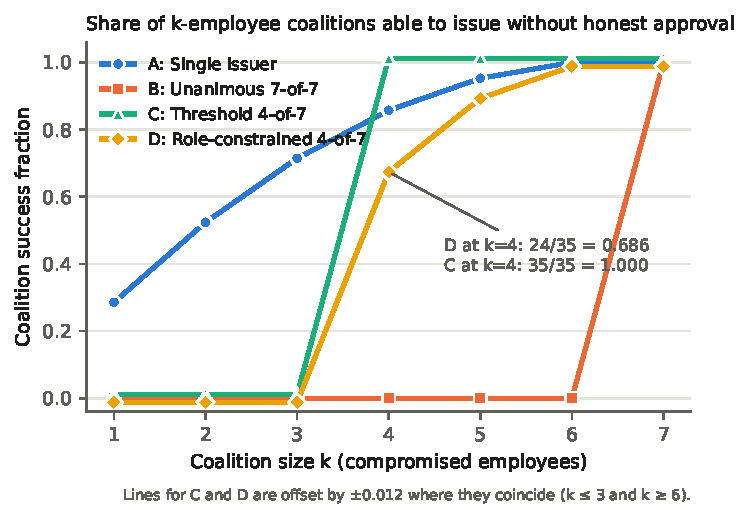
\includegraphics[width=\columnwidth]{fig_coalition}
\caption{Fraction of $k$-employee coalitions able to issue a credential without any honest approval.}
\label{fig:coalition}
\end{figure}

\begin{figure*}[t]
\centering
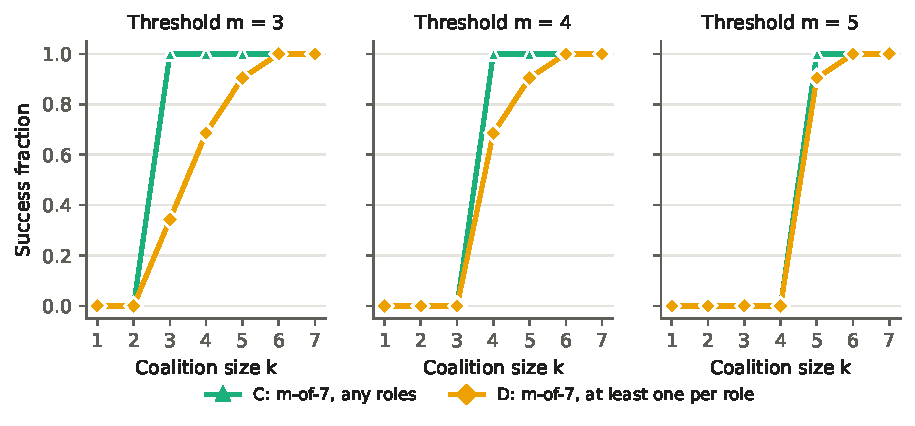
\includegraphics[width=0.85\textwidth]{fig_coalition_sensitivity}
\caption{Threshold policy (C) versus role-constrained policy (D) at thresholds 3, 4 and 5.}
\label{fig:coalition-sensitivity}
\end{figure*}

% Generated by experiments/generate_figures.py -- do not edit by hand.
\begin{table*}[t]
\centering
\small
\caption{Coalitions of $k$ employees able to issue, per policy (2 Registrars, 3 Deans, 2 Exam Officers).}
\label{tab:coalition}
\begin{tabular}{crrrr}
\hline
$k$ & A & B & C (4-of-7) & D (4-of-7, roles) \\
\hline
1 & 2/7 (0.286) & 0/7 (0.000) & 0/7 (0.000) & 0/7 (0.000) \\
2 & 11/21 (0.524) & 0/21 (0.000) & 0/21 (0.000) & 0/21 (0.000) \\
3 & 25/35 (0.714) & 0/35 (0.000) & 0/35 (0.000) & 0/35 (0.000) \\
4 & 30/35 (0.857) & 0/35 (0.000) & 35/35 (1.000) & 24/35 (0.686) \\
5 & 20/21 (0.952) & 0/21 (0.000) & 21/21 (1.000) & 19/21 (0.905) \\
6 & 7/7 (1.000) & 0/7 (0.000) & 7/7 (1.000) & 7/7 (1.000) \\
7 & 1/1 (1.000) & 1/1 (1.000) & 1/1 (1.000) & 1/1 (1.000) \\
\hline
\end{tabular}
\end{table*}


\note{Key facts to explain in your own words. Under A, a single insider suffices (\CoalAkOne{} of the single
employees). At threshold 4, role constraints leave the minimum coalition size unchanged (4) but reduce capable
4-person coalitions from \CoalCkFour{} to \CoalDkFour{} (\CoalDkFourFrac). The effect is larger at threshold 3
(\CoalCthreekThree{} vs.\ \CoalDthreekThree) and nearly vanishes at 5 (\CoalCfivekFive{} vs.\
\CoalDfivekFive). Why: with more required approvers, almost every coalition already spans all roles.}

\subsection{Gas consumption}
\begin{figure}[t]
\centering
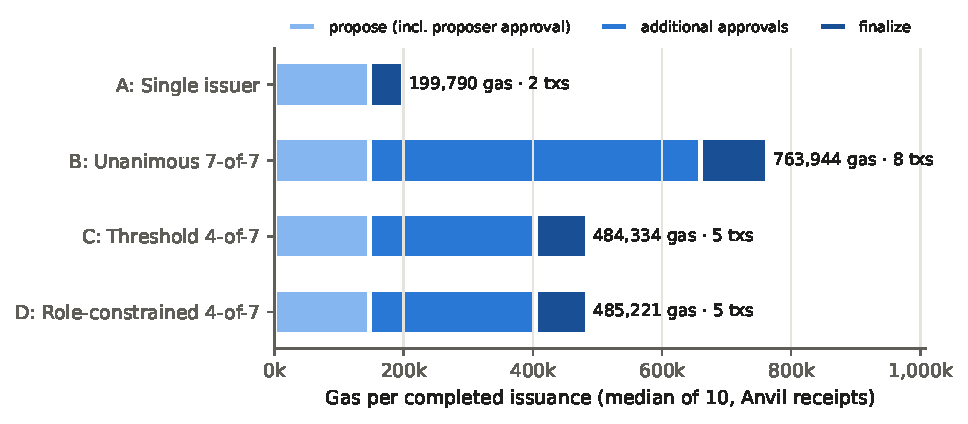
\includegraphics[width=\columnwidth]{fig_gas}
\caption{Gas per completed issuance (median of 10), split into proposal, additional approvals and finalization.}
\label{fig:gas}
\end{figure}

% Generated by experiments/generate_figures.py -- do not edit by hand.
\begin{table*}[t]
\centering
\small
\caption{Median gas from Anvil transaction receipts (10 issuances per policy).}
\label{tab:gas}
\begin{tabular}{lrrrr}
\hline
Operation & A & B & C & D \\
\hline
Deploy policy & 150,365 & 153,379 & 170,266 & 286,817 \\
Deploy registry & 2,615,457 & 2,615,457 & 2,615,457 & 2,615,457 \\
Add approver & 65,495 & 65,495 & 65,495 & 65,495 \\
Change role & 43,930 & 43,930 & 43,930 & 43,930 \\
(De)activate approver & 37,809 & 37,809 & 37,809 & 37,809 \\
Propose & 146,228 & 146,231 & 146,253 & 146,253 \\
Approve (each) & -- & 85,639 & 85,661 & 85,661 \\
Finalize & 53,562 & 103,879 & 81,098 & 81,985 \\
Revoke & 54,501 & 54,501 & 54,501 & 54,501 \\
Verify (eth\_call estimate) & 29,408 & 29,408 & 29,408 & 29,408 \\
\textbf{Total per issuance} & \textbf{199,790} & \textbf{763,944} & \textbf{484,334} & \textbf{485,221} \\
Transactions per issuance & 2 & 8 & 5 & 5 \\
\hline
\end{tabular}
\end{table*}


\note{Totals: A \GasTotalA, B \GasTotalB, C \GasTotalC, D \GasTotalD{} gas. The role check costs
\GasRoleOverhead{} gas (\GasRoleOverheadPct) per issuance, all in finalization (\GasFinalizeC{} vs.\
\GasFinalizeD). Cost scales with the number of approvals (\GasApproveEach{} gas each), not with the policy
logic.}

\subsection{Availability and delay}
\begin{figure*}[t]
\centering
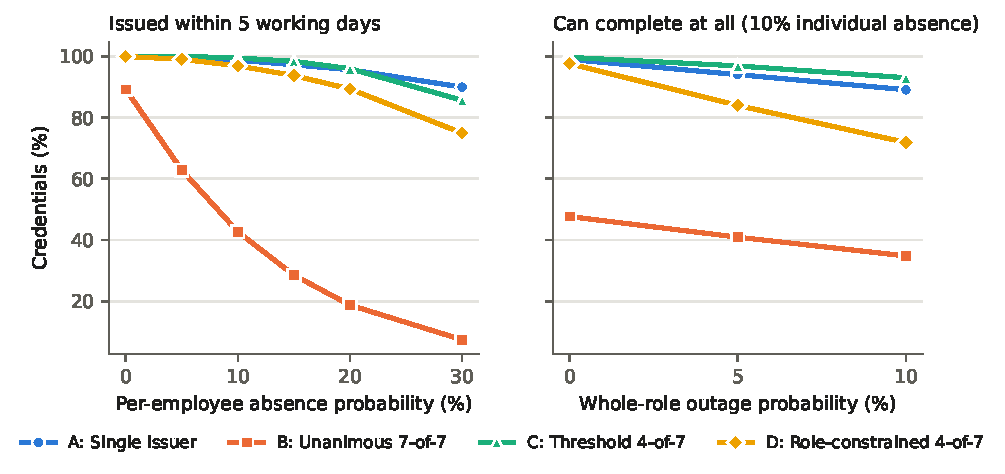
\includegraphics[width=0.85\textwidth]{fig_availability}
\caption{Left: credentials issued within 5 working days versus individual absence. Right: credentials that can
be issued at all versus the probability that an entire role is unavailable (10\% individual absence).
Simulated.}
\label{fig:availability}
\end{figure*}

\begin{figure*}[t]
\centering
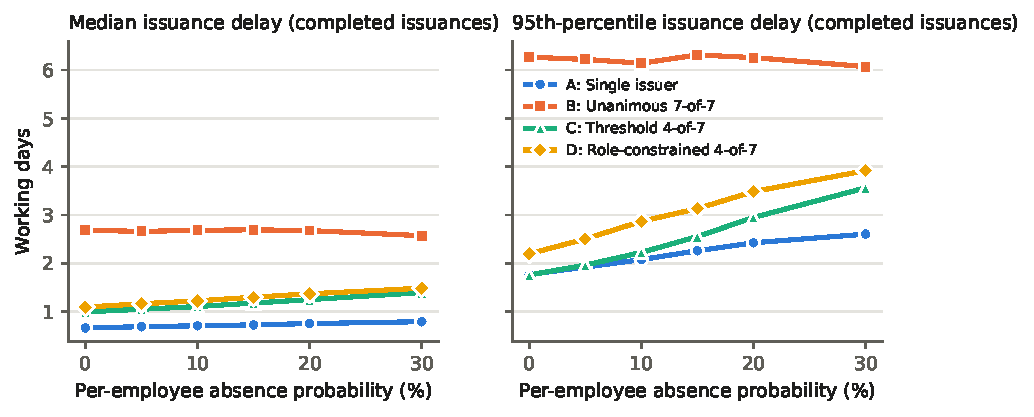
\includegraphics[width=0.85\textwidth]{fig_delay}
\caption{Median and 95th-percentile simulated issuance delay of completed issuances.}
\label{fig:delay}
\end{figure*}

% Generated by experiments/generate_figures.py -- do not edit by hand.
\begin{table}[t]
\centering
\small
\caption{Simulated workflow at 10\% individual absence (20{,}000 trials, seed 435, deadline 5 working days). Delays in working days over completed issuances.}
\label{tab:availability}
\begin{tabular}{lrrrrrr}
\hline
Policy & Completes & On time & Median & P95 & Cannot complete & of which: role \\
\hline
A: Single issuer & 99.0\% & 98.7\% & 0.71 & 2.08 & 1.0\% & 1.0\% \\
B: Unanimous 7-of-7 & 47.7\% & 42.7\% & 2.68 & 6.14 & 52.3\% & 0.0\% \\
C: Threshold 4-of-7 & 99.6\% & 99.5\% & 1.10 & 2.22 & 0.4\% & 0.0\% \\
D: Role-constrained 4-of-7 & 97.6\% & 96.9\% & 1.22 & 2.87 & 2.4\% & 2.1\% \\
\hline
\end{tabular}
\end{table}


\note{At 10\% absence, on-time issuance is A \OnTimeA, B \OnTimeB, C \OnTimeC, D \OnTimeD. D's extra failures
are caused by a missing role (\MissingRoleD{} of trials). Under a 5\% whole-role outage, D completes
\OutageFiveD{} versus \OutageFiveC{} for C (at 10\%: \OutageTenD{} versus \OutageTenC). Unanimous is
impractical (\CompleteB{} completion).}

\subsection{Security--cost--availability trade-off}
\begin{figure}[t]
\centering
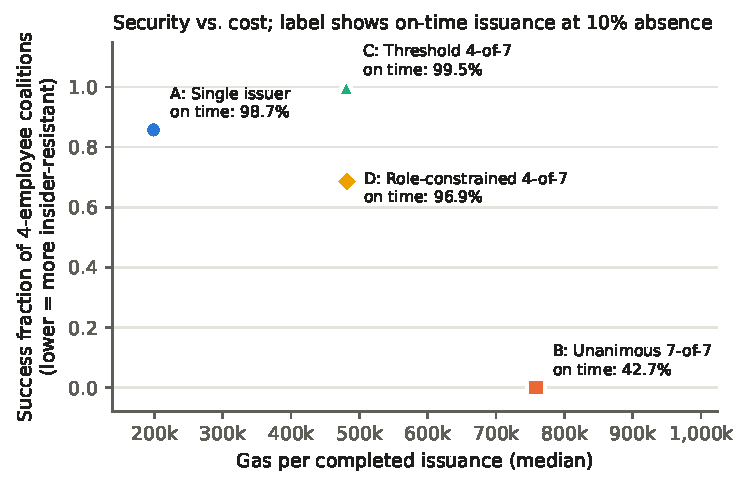
\includegraphics[width=\columnwidth]{fig_tradeoff}
\caption{Coalition exposure at $k=4$ versus gas per issuance; labels give on-time issuance at 10\% absence.}
\label{fig:tradeoff}
\end{figure}
\note{One paragraph that answers the research question directly. No policy dominates on all three axes.}

\section{Deployment in Kazakhstan: A Hypothetical Case}\label{sec:kz}
We discuss how such a registry might relate to existing practice, with Nazarbayev University (NU) as a hypothetical institution. NU does not use this system, we have no data on its internal approval workflow, and recording a commitment does not by itself give a diploma legal recognition.

\subsection{Existing infrastructure}
The Unified Platform of Higher Education (EPVO) is a national database of the Ministry of Science and Higher Education covering institutions, programs, staff and students~\cite{epvo}. In August 2026 the Ministry described the current process: diplomas are generated in a special module that assigns a unique number and QR code, access is limited to officially responsible university staff registered in the module, and no number can be generated for a student without an EPVO record~\cite{kznews2026}. An employer can check a diploma at the EPVO portal using its number, its series and the holder's individual identification number, and may contact the university when no record is found~\cite{kzfaq}.

Two points follow. The weaknesses described in the 2023 report should not be presented as current practice, because the Ministry has since described restricted access. Restricting access does not necessarily divide authority, however. The public description does not say how many responsible employees must agree before a diploma is generated, and we do not know the internal rule. This is the question our policies address.

\subsection{Complementing EPVO}
EPVO would remain the authoritative register. A commitment registry could add independent evidence of who approved a record and when, and make later removal or change of that evidence visible. One option is that a university collects approvals in the registry before the EPVO module generates the number; another is that EPVO publishes commitments for diplomas it already holds, which would provide tamper evidence without multi-party approval. Either would need a decision by the Ministry and integration work that we have not done.

Integration of this kind has been prototyped: Ussatova et al.\ describe an application that draws historical transcript and diploma data from the national platform, and note that the state data exchange they use does not verify grades, transcript entries or diploma numbers~\cite{ussatova2026b}.

\subsection{Roles and governance}
Mapping roles to a university is an institutional choice. Our example combines the registrar's office, schools and examination officers, similar in spirit to the suggestion in Cerberus~\cite{tariq2023}. With two examination officers, their simultaneous absence stops all issuance under D. Experiment D shows that a third holder largely solves individual absence, but not the closure of an office during an examination period. That case needs a formal rule for substitution between offices, and a substitute who acts for two roles weakens the separation.

The governor is the most sensitive position. Options include the Ministry, a group of universities, or a multisignature account with a time delay; OpenZeppelin documents timelocks and multisignature owners for such cases~\cite{ozdocs}. Placing the governor inside the same office as the approvers would undo the separation.

\subsection{Legal status}
Under the Law on Education, documents of education are of state form, of an institution's own form, or issued by autonomous organizations of education, and documents of the last kind are treated as equal to state-form documents~\cite{kzedu}. Autonomous organizations determine the form of their own documents~\cite{kzedu}. Which category applies to a given institution would have to be confirmed before deployment. The Ministry states that own-form documents without a generated number and QR code are considered invalid~\cite{kznews2026}. An on-chain record therefore cannot replace the official procedure.

\subsection{Personal data}
The Law on Personal Data defines personal data as information about a subject supplemented by one or more identifiers, and defines an identifier broadly enough to include information that links data sets about a person~\cite{kzdata}. Four provisions bear directly on a public chain. Personal data must be stored in a database or digital object located in Kazakhstan (Article 12). Cross-border transfer is allowed to states that protect personal data, and otherwise in listed cases such as consent (Article 16). Data must be destroyed or deleted in listed cases (Article 18), and subjects may request changes and, in certain cases, deletion (Article 24)~\cite{kzdata}.

The law mentions hashing as a method of protecting personal data, and separately defines anonymization as an irreversible transformation of identifiers after which attribution to a subject is impossible~\cite{kzdata}. In the provisions we read, we found no statement on whether a salted commitment is personal data. European guidance, which is not binding in Kazakhstan, is strict on this point: the European Data Protection Board states that a salted or keyed hash of personal data is itself considered personal data, while noting that after deletion of the salt or key the hash should not be linkable to the original data, provided that the algorithm is not broken and the salt did not leak~\cite{edpb2025}. The same guidelines say that unsalted hashes are in general not sufficient on a public blockchain, and that the lifetime of the chain should not be assumed to be an appropriate retention period (paragraphs 52 and 78)~\cite{edpb2025}. Our design follows the first point. It does not resolve the second: the registry has no deletion, so destroying the off-chain document and every copy of the salt is the only available measure, and a holder who keeps a copy cannot be made to destroy it. We therefore do not call commitments anonymous. If they are personal data, replication on foreign nodes raises the storage and transfer rules above. A permissioned network hosted in Kazakhstan could reduce part of this problem but would concentrate trust in its operators. Legal advice is required.

\subsection{Cost}
Deploying the registry costs \GasDeployRegistry{} gas, adding an approver about \GasAddApprover{}, and revocation \GasRevoke{}. Issuance under D costs \GasTotalD{} gas. The monetary cost depends on the gas price and exchange rate, which we did not measure. At illustrative prices of 0.5 and 30~gwei, one issuance would cost \EthLowD{} and \EthHighD{}~ETH. Key management, staff training and integration with EPVO are additional costs that gas figures do not show. Committing to several credentials in one Merkle root, as Cerberus does per batch~\cite{tariq2023}, would reduce cost per credential; we did not implement it.

\subsection{What the system cannot prevent}
If a false grade or student record already exists when the proposal is made, every policy can issue the resulting diploma. Multi-party approval helps only if approvers check the source record independently. If all of them trust the same database entry, four signatures may represent one error. The system shows who authorized a credential and not that its content is true.

\section{Discussion and Limitations}\label{sec:discussion}
% Required by the course. Name the real weaknesses plainly.

\note{Interpretation: role separation is a cheap filter on coalitions, not a stronger threshold. If the goal is
a higher minimum number of insiders, raise the threshold. If the goal is to force collusion across departments,
add role constraints, and plan for role availability (more than one holder per role, delegation rules).}

\note{Limitations (see docs/THREAT\_MODEL.md and docs/EXPERIMENTS.md):
(1) the governor is trusted; a compromised governor can add approver keys and satisfy any policy;
(2) revocation is single-party, identical across policies by design;
(3) only one 7-person configuration was studied; results depend on role sizes;
(4) the coalition success fraction is not a fraud probability;
(5) simulation parameters are assumptions, not measured NU workflows;
(6) local Anvil only, no testnet or mainnet fees measured; gas prices in \texttt{gas\_cost\_eth.csv} are
assumptions;
(7) proposals never expire, and front-running griefing is possible;
(8) blockchain cannot detect falsified source records;
(9) metadata is public (approver addresses, timing).}

\section{Conclusion}\label{sec:conclusion}
We compared four rules for authorizing academic credentials within one smart-contract design. At a common 4-of-7 threshold, requiring a registrar, a dean and an examination officer did not increase the number of insiders needed. It excluded \BlockCoalExcluded{} of the 35 coalitions of that size and cost \GasRoleOverhead{} additional gas per issuance. It also reduced the number of absences that can block issuance from four to two, and lowered simulated completion from \OutageFiveC{} to \OutageFiveD{} under a 5\% whole-role outage. Additional holders of each role reduced the loss from individual absence and not from whole-role outages. The benefit of roles was modest under independent compromise and large when collusion was correlated within offices. A single issuer is cheap but fails with one insider. Unanimity resists every coalition smaller than the whole group but is rarely available.

Role constraints are therefore best seen as a way to require collusion across offices and not as a substitute for a higher threshold, and they should be accompanied by enough holders of each role. Future work should remove reliance on one governor, study conditional delegation, replace assumed collusion patterns by evidence, replace assumed delays by observed ones, require several parties for revocation, and test the system on a public or permissioned network. None of these changes would by itself establish that the source record is true.


\section*{Code and Data Availability}
The contracts are built with Foundry~\cite{foundry,forgestd} and OpenZeppelin Contracts~\cite{openzeppelin2024}.
All code, data, figures and tables are reproducible with
\texttt{python experiments/run\_all.py} from
\url{https://github.com/VeyelutD/education-credential-verification}.

\bibliographystyle{IEEEtran}
\bibliography{references}

\end{document}
